% Methodology section

\subsection{Operads}

A large class of mathematical theories consists of three ingredients:
\begin{enumerate}
  \item A collection of objects.
  \item A collection of morphisms between these objects.
  \item A notion of composition of these morphisms.
\end{enumerate}

The most well-known example of this pattern is arithmetic, where the objects are numbers, the morphisms are functions (addition, multiplication, etc.), and the composition is the usual function composition. All fields such as real numbers, complex numbers, and vector spaces can be described in this way.

As we go up the hierarchy of mathematics, we find more and more examples of this pattern. For example, in topology, the objects are topological spaces, the morphisms are continuous functions, and the composition is the usual function composition. Groups and family (magma, monoid, group, ring, field) are also examples of this pattern. Category theory is a generalization of this pattern, where the objects are categories, the morphisms are functors, and the composition is the usual functor composition.

Operads are a generalization of this pattern, where the objects are operations, the morphisms are operations of different arities, and the composition is a more general form of function composition. Operads provide a framework for studying algebraic structures that arise in various areas of mathematics, including topology, algebra, and category theory.

Operads consists of:

\begin{enumerate}
  \item A collection of operations of different arities.
  \item A notion of composition of these operations.
  \item The composition operations obey certain conditions - associativity and unitality.
\end{enumerate}

\textbf{Formal Definition}
\\

Consider a set $\mathbb{X}$, and an integer $n \in \mathbb{N}$.

An Operad, $\mathbb{P}$, is defined as a set of n-ary operations, where each operation $f$ has the signature $\mathbb{X}^n \to \mathbb{X}$:

\begin{equation}
  \mathbb{P}(n) = \{f: \mathbb{X}^n \to \mathbb{X}\}
\end{equation}

where $\mathbb{X}^n$ is the cartesian product of $\mathbb{X}$ with itself $n$ times, i.e.

\begin{equation}
  \mathbb{X}^n = \mathbb{X} \times \mathbb{X} \times \ldots \times \mathbb{X}
\end{equation}

i.e. all of these functions $f$ take in $n$ arguments from $\mathbb{X}$ and return a single element from $\mathbb{X}$.

\begin{figure}[h]
\centering
    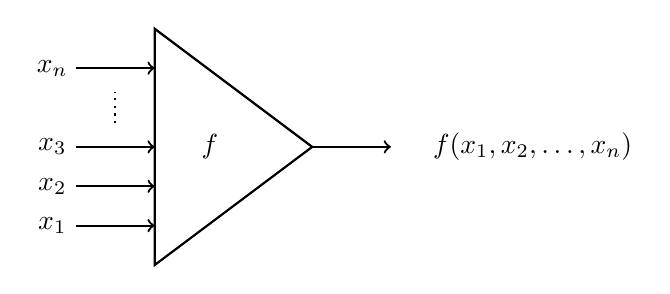
\begin{tikzpicture}
        % Draw the triangle with vertical left edge
        \draw[thick, fill=white] (0,0) -- (0,3) -- (2,1.5) -- cycle;

        % Draw input arrows
        \draw[->, thick] (-1,0.5) -- (0,0.5);
        \draw[->, thick] (-1,1) -- (0,1);
        \draw[->, thick] (-1,1.5) -- (0,1.5);
        \draw[dotted, thick] (-0.5,1.8) -- (-0.5,2.2);
        \draw[->, thick] (-1,2.5) -- (0,2.5);

        % Draw output arrow
        \draw[->, thick] (2,1.5) -- (3,1.5);

        % Add labels
        \node at (0.7,1.5) {$f$};
        \node at (-1.3,0.5) {$x_1$};
        \node at (-1.3,1) {$x_2$};
        \node at (-1.3,1.5) {$x_3$};
        \node at (4.8,1.5) {$f(x_1,x_2,\ldots,x_n)$};
        \node at (-1.3,2.5) {$x_n$};
    \end{tikzpicture}
\end{figure}

If we have a bunch of these sets of functions $\mathbb{P}(k_i)$ for each $k_i \in \mathbb{N}$, then we can define a composition operation $\circ$ for these operations as follows:

Let $f_i \in \mathbb{P}(k_i)$ be an operation that takes in $k_i$ arguments from $\mathbb{X}$ and returns a single element from $\mathbb{X}$. We can take n numbers of such operations and use their outputs as inputs to another operation $f \in \mathbb{P}(n)$, which takes in $n$ arguments from $\mathbb{X}$ and returns a single element from $\mathbb{X}$. The composition operation $\circ$ is defined as:

\begin{equation}
    \mathbb{P}(n) \times ( \mathbb{P}(k_1) \times \mathbb{P}(k_2) \times \ldots \times \mathbb{P}(k_n) ) \to \mathbb{P}(k_1 + k_2 + \ldots + k_n)
\end{equation}

\begin{equation}
    f, (f_1, f_2, \ldots, f_n) \mapsto f \circ (f_1, f_2, \ldots, f_n)
\end{equation}

where $f \circ (f_1, f_2, \ldots, f_n) \in \mathbb{P}(k_1 + k_2 + \ldots + k_n)$ is defined as the following diagram:

\begin{figure}[h]
\centering
\begin{tikzpicture}[scale=0.9]
    % Main operation triangle
    \draw[thick, fill=white] (0,0) -- (0,5.5) -- (4,2.75) -- cycle;
    \node at (1.5,2.75) {$f$};

    % First sub-operation triangle
    \draw[thick, fill=white] (-5,0) -- (-5,1.5) -- (-3,0.75) -- cycle;
    \node at (-4.3,0.75) {$f_1$};

    % Second sub-operation triangle
    \draw[thick, fill=white] (-5,2) -- (-5,3.5) -- (-3,2.75) -- cycle;
    \node at (-4.3,2.75) {$f_2$};

    % Third sub-operation triangle (with dotted line indicating more)
    \draw[thick, fill=white] (-5,4) -- (-5,5.5) -- (-3,4.75) -- cycle;
    \node at (-4.3,4.75) {$f_n$};

    % Dotted line between second and third triangles
    \draw[dotted, thick] (-4,3.7) -- (-4,4);

    % Input arrows for first sub-operation
    \draw[->, thick] (-7,0.25) -- (-5,0.25);
    \draw[->, thick] (-7,0.75) -- (-5,0.75);
    \draw[->, thick] (-7,1.25) -- (-5,1.25);
    \node at (-8.4,0.25) {$x_1}$};
    \node at (-8.4,0.75) {$\ldots$};
    \node at (-8.4,1.25) {$x_{k_1}$};

    % Input arrows for second sub-operation
    \draw[->, thick] (-7,2.25) -- (-5,2.25);
    \draw[->, thick] (-7,2.75) -- (-5,2.75);
    \draw[->, thick] (-7,3.25) -- (-5,3.25);
    \node at (-8.4,2.25) {$x_{k_1+1}}$};
    \node at (-8.4,2.75) {$\ldots$};
    \node at (-8.4,3.25) {$x_{k_1+k_2}$};

    % Input arrows for third sub-operation
    \draw[->, thick] (-7,4.25) -- (-5,4.25);
    \draw[->, thick] (-7,4.75) -- (-5,4.75);
    \draw[->, thick] (-7,5.25) -- (-5,5.25);
    \node at (-8.4,4.25) {$x_{k_1+...+k_{n-1}+1}$};
    \node at (-8.4,4.75) {$\ldots$};
    \node at (-8.4,5.25) {$x_{k_1+...+k_{n-1}+k_n}$};

    % Connecting arrows from sub-operations to main operation
    \draw[->, thick] (-3,0.75) -- (0,0.75);
    \draw[->, thick] (-3,2.75) -- (0,2.75);
    \draw[->, thick] (-3,4.75) -- (0,4.75);

    % Output arrow
    \draw[->, thick] (4,2.75) -- (6,2.75);

    % Final output label
    \node at (6,3.5) {$f \circ (f_1, f_2, \ldots, f_n)$};

    % Dotted lines to indicate more inputs for each sub-operation
    \draw[dotted, thick] (-6,1) -- (-6,1.1);
    \draw[dotted, thick] (-6,3) -- (-6,3.1);
    \draw[dotted, thick] (-6,4.5) -- (-6,4.6);

\end{tikzpicture}
\caption{Operadic composition showing how multiple operations $f_1, f_2, \ldots, f_n$ with arities $k_1, k_2, \ldots, k_n$ can be composed with an operation $f$ of arity $n$ to form a new operation of arity $k_1 + k_2 + \ldots + k_n$.}
\label{fig:operadic-composition}
\end{figure}

Associativity of this composition for Operads works as follows:

\begin{figure}[h]
\centering
    \begin{tikzpicture}[grow'=up]
        \begin{scope}[xshift=-5cm]
            \node {(ab)c}
            child {
                node {ab}
                child {
                    node {a}
                }
                child {
                    node {b}
                }
            }
            child{
                node {c}
            };
        \end{scope}
        \begin{scope}[xshift=0cm]
            \node {(ab)c}
            child{
                node {a}
            }
            child {
                node {bc}
                    child {
                node {b}
                }
                child {
                    node {c}
                }
            };
        \end{scope}
        \begin{scope}[xshift=5cm]
            \node {abc}
            child{
                node {a}
            }
            child {
                node {b}
            }
            child {
                node {c}
            };
        \end{scope}
    \end{tikzpicture}
    \caption{Associativity of operadic composition of arity 3}
\end{figure}

\begin{figure}[h]
\centering
\begin{tikzpicture}[grow'=up, level distance=1.5cm, sibling distance=2cm]
    % First tree: ((ab)c)d
    \begin{scope}[xshift=-10cm]
        \node {((ab)c)d}
        child {
            node {(ab)c}
            child {
                node {ab}
                child {
                    node {a}
                }
                child {
                    node {b}
                }
            }
            child {
                node {c}
            }
        }
        child {
            node {d}
        };
    \end{scope}

    % Second tree: (a(bc))d
    \begin{scope}[xshift=-5cm]
        \node {(a(bc))d}
        child {
            node {a(bc)}
            child {
                node {a}
            }
            child {
                node {bc}
                child {
                    node {b}
                }
                child {
                    node {c}
                }
            }
        }
        child {
            node {d}
        };
    \end{scope}

    % Third tree: (ab)(cd)
    \begin{scope}[yshift=6cm, xshift=0cm]
        \node {(ab)(cd)}
        child {
            node {ab}
            child {
                node {a}
            }
            child {
                node {b}
            }
        }
        child {
            node {cd}
            child {
                node {c}
            }
            child {
                node {d}
            }
        };
    \end{scope}

    % Fourth tree: a((bc)d)
    \begin{scope}[yshift=6cm, xshift=-10cm]
        \node {a((bc)d)}
        child {
            node {a}
        }
        child {
            node {(bc)d}
            child {
                node {bc}
                child {
                    node {b}
                }
                child {
                    node {c}
                }
            }
            child {
                node {d}
            }
        };
    \end{scope}

    % Fifth tree: a(b(cd))
    \begin{scope}[yshift=6cm, xshift=-5cm]
        \node {a(b(cd))}
        child {
            node {a}
        }
        child {
            node {b(cd)}
            child {
                node {b}
            }
            child {
                node {cd}
                child {
                    node {c}
                }
                child {
                    node {d}
                }
            }
        };
    \end{scope}

    \begin{scope}
        \node {abcd}
        child {
            node {a}
        }
        child {
            node {b}
        }
        child {
            node {c}
        }
        child {
            node {d}
        };
    \end{scope}

\end{tikzpicture}
\caption{Associativity of operadic composition of arity 4}
\label{fig:arity-4-associativity}
\end{figure}

This composition operation $\circ$ satisfies the following properties:

\begin{itemize}
  \item \textbf{Associativity}: For all $f \in \mathbb{P}(n)$, $g \in \mathbb{P}(k_1)$, $h \in \mathbb{P}(k_2)$, and $i \in \mathbb{P}(k_3)$, we have:

  \begin{equation}
    f \circ (g \circ (h, i)) = (f \circ (g, h)) \circ i
  \end{equation}

  \item \textbf{Unitality}: For all $f \in \mathbb{P}(n)$, we have:

  \begin{equation}
    f \circ (\text{id}_{k_1}, \text{id}_{k_2}, \ldots, \text{id}_{k_n}) = f
  \end{equation}

  where $\text{id}_k$ is the identity function on $\mathbb{X}^k$.
\end{itemize}

Symmetry is not required for operads, but it can be added to form symmetric operads. The symmetry condition is:

\begin{equation}
  f \circ (g_1, g_2, \ldots, g_n) = f \circ (g_{\sigma(1)}, g_{\sigma(2)}, \ldots, g_{\sigma(n)})
\end{equation}

where $\sigma$ is a permutation of the set $\{1, 2, \ldots, n\}$ or $\sigma \in S_n$ and $g_{\sigma(i)}$ is the $\sigma(i)$-th element of the original sequence, i.e., the permutation $\sigma$ permutes the order of operations used as inputs to $f$.

\subsubsection{T-operads}

T-operads, or typed operads, extend the concept of operads by introducing a typing system, making them particularly suitable for modeling complex systems with heterogeneous components and interactions. Unlike standard operads where all operations have the same domain and codomain, T-operads allow for typed inputs and outputs, enabling more precise representation of systems with different types of entities and their interactions.

\textbf{Formal Definition}
\\

A T-operad consists of:

\begin{enumerate}
  \item A set of types $T = \{t_1, t_2, \ldots, t_m\}$
  \item For each sequence of input types $\mathbf{s} = (s_1, s_2, \ldots, s_n)$ where each $s_i \in T$, and an output type $t \in T$, a set of operations $\mathbb{P}(\mathbf{s}; t)$
  \item A composition operation that respects types
\end{enumerate}

More formally, let $T$ be a set of types. A T-operad $\mathbb{P}$ assigns to each sequence of input types $\mathbf{s} = (s_1, s_2, \ldots, s_n)$ and output type $t$ a set $\mathbb{P}(\mathbf{s}; t)$ of operations that take inputs of types $s_1, s_2, \ldots, s_n$ and produce an output of type $t$:

\begin{equation}
  \mathbb{P}(\mathbf{s}; t) = \{f: s_1 \times s_2 \times \ldots \times s_n \rightarrow t\}
\end{equation}

\begin{figure}[h]
\centering
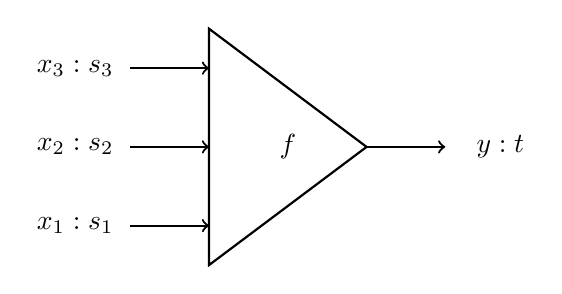
\begin{tikzpicture}
    % Draw the triangle with vertical left edge
    \draw[thick, fill=white] (0,0) -- (0,3) -- (2,1.5) -- cycle;

    % Draw input arrows
    \draw[->, thick] (-1,0.5) -- (0,0.5);
    \draw[->, thick] (-1,1.5) -- (0,1.5);
    \draw[->, thick] (-1,2.5) -- (0,2.5);

    % Draw output arrow
    \draw[->, thick] (2,1.5) -- (3,1.5);

    % Add labels
    \node at (1,1.5) {$f$};
    \node at (-1.7,0.5) {$x_1: s_1$};
    \node at (-1.7,1.5) {$x_2: s_2$};
    \node at (-1.7,2.5) {$x_3: s_3$};
    \node at (3.7,1.5) {$y: t$};
\end{tikzpicture}
\caption{A typed operation $f \in \mathbb{P}((s_1, s_2, s_3); t)$ taking three inputs of potentially different types and producing an output of type $t$.}
\label{fig:typed-operation}
\end{figure}

The composition operation must respect the typing constraints. Given operations:
\begin{itemize}
  \item $f \in \mathbb{P}((t_1, t_2, \ldots, t_n); t)$
  \item $g_1 \in \mathbb{P}(\mathbf{s}_1; t_1)$
  \item $g_2 \in \mathbb{P}(\mathbf{s}_2; t_2)$
  \item $\ldots$
  \item $g_n \in \mathbb{P}(\mathbf{s}_n; t_n)$
\end{itemize}

The composition $f \circ (g_1, g_2, \ldots, g_n)$ is defined only when the output type of each $g_i$ matches the corresponding input type required by $f$. The resulting operation has input types given by the concatenation of all input types of the $g_i$ operations and output type $t$:

\begin{equation}
  f \circ (g_1, g_2, \ldots, g_n) \in \mathbb{P}(\mathbf{s}_1 \cdot \mathbf{s}_2 \cdot \ldots \cdot \mathbf{s}_n; t)
\end{equation}

where $\cdot$ denotes concatenation of type sequences.

\begin{figure}[h]
\centering
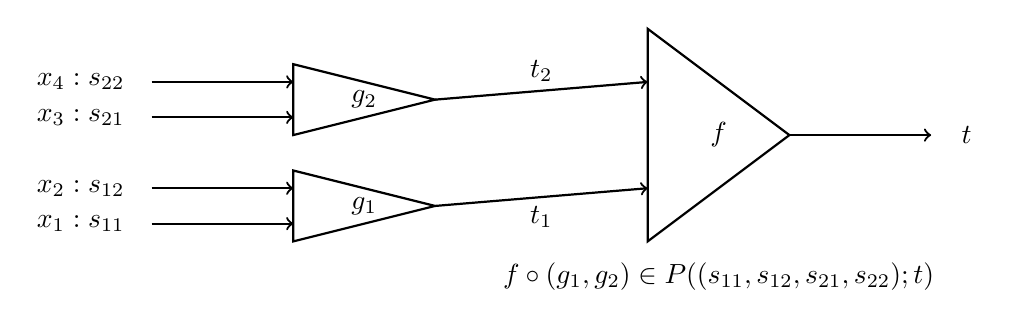
\begin{tikzpicture}[scale=0.9]
    % Main operation triangle
    \draw[thick, fill=white] (0,0) -- (0,3) -- (2,1.5) -- cycle;
    \node at (1,1.5) {$f$};

    % First sub-operation triangle
    \draw[thick, fill=white] (-5,0) -- (-5,1) -- (-3,0.5) -- cycle;
    \node at (-4,0.5) {$g_1$};

    % Second sub-operation triangle
    \draw[thick, fill=white] (-5,1.5) -- (-5,2.5) -- (-3,2) -- cycle;
    \node at (-4,2) {$g_2$};

    % Input arrows for first sub-operation
    \draw[->, thick] (-7,0.25) -- (-5,0.25);
    \draw[->, thick] (-7,0.75) -- (-5,0.75);
    \node at (-8,0.25) {$x_1: s_{11}$};
    \node at (-8,0.75) {$x_2: s_{12}$};

    % Input arrows for second sub-operation
    \draw[->, thick] (-7,1.75) -- (-5,1.75);
    \draw[->, thick] (-7,2.25) -- (-5,2.25);
    \node at (-8,1.75) {$x_3: s_{21}$};
    \node at (-8,2.25) {$x_4: s_{22}$};

    % Connecting arrows from sub-operations to main operation
    \draw[->, thick] (-3,0.5) -- (0,0.75);
    \node at (-1.5,0.35) {$t_1$};
    \draw[->, thick] (-3,2) -- (0,2.25);
    \node at (-1.5,2.4) {$t_2$};

    % Output arrow
    \draw[->, thick] (2,1.5) -- (4,1.5);
    \node at (4.5,1.5) {$t$};

    % Final composition label
    \node at (1,-0.5) {$f \circ (g_1, g_2) \in \mathbb{P}((s_{11}, s_{12}, s_{21}, s_{22}); t)$};
\end{tikzpicture}
\caption{Typed operadic composition showing how the output types of $g_1$ and $g_2$ must match the input types required by $f$.}
\label{fig:typed-operadic-composition}
\end{figure}

\textbf{Applications of T-operads to Complex Systems}
\\

T-operads provide several key advantages for modeling complex systems:

\begin{enumerate}
  \item \textbf{Heterogeneous Systems}: T-operads can model systems with different types of components, such as cells of different types in biological tissues, different species in ecological networks, or various agent types in economic systems.

  \item \textbf{Type-Restricted Interactions}: They capture the reality that not all elements can interact with all others—proteins can only bind to compatible partners, economic agents have specific roles, and neural signals have specific receptor requirements.

  \item \textbf{Phase Transitions}: Changes in the type structure of a T-operad can model fundamental shifts in system behavior. For example, the differentiation of stem cells involves changes in the types of operations available as cells specialize, and phase transitions in social systems correspond to changes in the roles individuals can play.

  \item \textbf{Hierarchical Organization}: T-operads naturally represent hierarchical systems where higher-level entities emerge from compositions of lower-level entities, potentially with type transformations occurring during composition.
\end{enumerate}

In biological systems, T-operads can represent protein interactions where specific protein types can only bind with compatible partners, forming complexes that then have new binding capabilities. In neural networks, T-operads can model how different neuron types (excitatory, inhibitory) combine to form functional circuits with specific input-output behaviors. In social systems, T-operads can represent how individuals with different expertise (types) combine to form organizations with emergent capabilities.

\textbf{Detecting Phase Transitions with T-operads}
\\

Phase transitions in complex systems can be identified through changes in the type structure of T-operads:

\begin{enumerate}
  \item \textbf{Type Emergence}: New types appear in the system, indicating new functionalities or states have emerged.

  \item \textbf{Compositional Reorganization}: Changes in which operation types can compose with each other, signaling a restructuring of system interactions.

  \item \textbf{Type Collapse}: Multiple types merge into a single type, indicating a loss of differentiation or specialization.

  \item \textbf{Connectivity Changes}: Alterations in the graph of possible type compositions, which can indicate critical transitions in system behavior.
\end{enumerate}

For example, in a financial system modeled with T-operads, a phase transition from stability to crisis might be detected by:
\begin{itemize}
  \item New operation types emerging (representing novel, risky financial instruments)
  \item Changes in which institution types can interact with which financial product types
  \item Collapse of previously distinct risk categories into correlated failure modes
\end{itemize}

These changes in the T-operad structure provide early warning signals for system-wide transitions that may not be detectable using traditional network or simplicial complex approaches.

\begin{figure}[h]
\centering
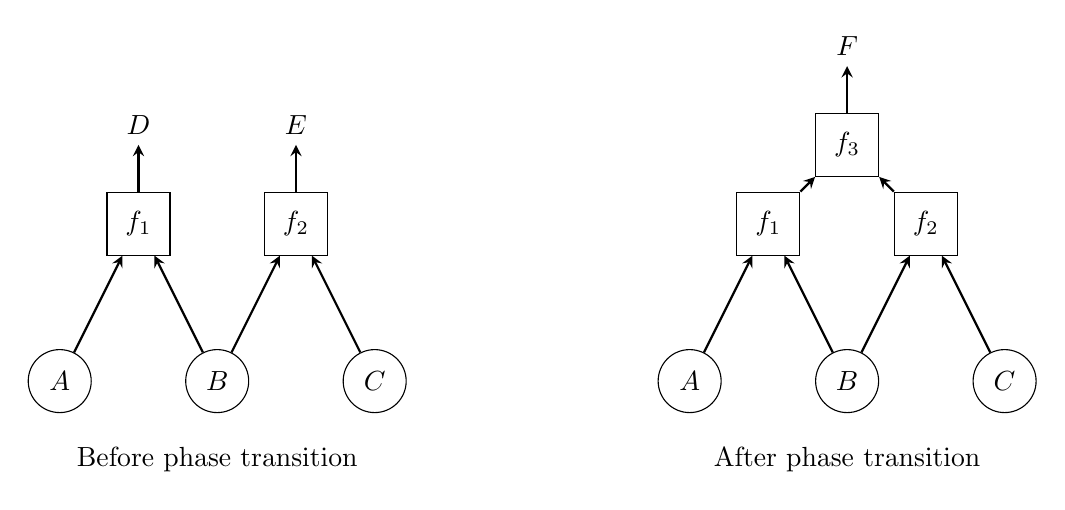
\begin{tikzpicture}[
    type/.style={circle, draw=black, fill=white, minimum size=0.8cm},
    op/.style={rectangle, draw=black, fill=white, minimum size=0.8cm},
    arr/.style={->, >=stealth, thick}
]
    % Before phase transition
    \begin{scope}[xshift=-6cm]
        % Types
        \node[type] (A1) at (0,0) {$A$};
        \node[type] (B1) at (2,0) {$B$};
        \node[type] (C1) at (4,0) {$C$};

        % Operations
        \node[op] (op1) at (1,2) {$f_1$};
        \node[op] (op2) at (3,2) {$f_2$};

        % Arrows
        \draw[arr] (A1) -- (op1);
        \draw[arr] (B1) -- (op1);
        \draw[arr] (op1) -- (1,3) node[above] {$D$};

        \draw[arr] (B1) -- (op2);
        \draw[arr] (C1) -- (op2);
        \draw[arr] (op2) -- (3,3) node[above] {$E$};

        \node at (2,-1) {Before phase transition};
    \end{scope}

    % After phase transition
    \begin{scope}[xshift=2cm]
        % Types
        \node[type] (A2) at (0,0) {$A$};
        \node[type] (B2) at (2,0) {$B$};
        \node[type] (C2) at (4,0) {$C$};

        % Operations
        \node[op] (op3) at (1,2) {$f_1$};
        \node[op] (op4) at (3,2) {$f_2$};
        \node[op] (op5) at (2,3) {$f_3$}; % New operation

        % Arrows
        \draw[arr] (A2) -- (op3);
        \draw[arr] (B2) -- (op3);
        \draw[arr] (op3) -- (op5);

        \draw[arr] (B2) -- (op4);
        \draw[arr] (C2) -- (op4);
        \draw[arr] (op4) -- (op5);

        \draw[arr] (op5) -- (2,4) node[above] {$F$}; % New type

        \node at (2,-1) {After phase transition};
    \end{scope}
\end{tikzpicture}
\caption{Phase transition in a T-operad: Before the transition, operations $f_1$ and $f_2$ produce different types. After the transition, a new composition capability emerges with operation $f_3$ that can take outputs from both $f_1$ and $f_2$ to produce a new type $F$.}
\label{fig:typed-phase-transition}
\end{figure}

T-operads thus provide a powerful framework for modeling complex systems where the types of interactions and entities matter, enabling us to detect and analyze phase transitions that involve changes in the system's compositional structure and typing relationships.

